\chapter{Natural Language Processing}
\label{chap:nlp}

\section{Machine Learning}
\label{sec:ml}

\subsection{Textbereinigung und Vorverarbeitung}
\label{sec:text_vorverarbeitung}

%TODO: Einleitung oder entfernen!

\begin{itemize}
    \item \textbf{Titel und Inhalt der Artikel zusammenfügen \cite{Buddhadev2025}}: Damit keine wichtigen Informationen verloren gehen,
    werden Titel und Inhalt des Artikels zusammengefasst. Gerade der Titel kann durch z.B. Clickbait (siehe \ref{sec:wie_definieren_sich_fake_news})
    schnell Hinweise auf eventuelle Fake News geben.

    \item \textbf{Akzente und Sonderzeichen entfernen \cite{Buddhadev2025} \cite{sabir2025} \cite{aslam2022}}: Akzente führen dazu, dass Wörter wie „café“ und „cafe“ unterschiedlich behandelt werden, 
    obwohl sie semantisch gleich sind. Das Entfernen dieser erhöht die Generalisierung. Sonderzeichen stören einfache Tokenizer (z. B. bei Bag-of-Words), führen zu vielen seltenen Tokens und zu 
    überdimensionierten Vektoren (siehe \ref{sec:bag_of_words}).

    \item \textbf{Alle Buchstaben zu Kleinbuchstaben konvertieren \cite{sabir2025} \cite{SUDHAKAR2024101028} \cite{aslam2022}}: Ähnlich wie zum vorherigen Punkt
    erhöht die durchgehende Kleinschreibung aller Buchstaben die Generalisierung und verhindert somit unnötige Duplikate im Vokabular.

    \item \textbf{Leere Spalten entfernen \cite{SUDHAKAR2024101028}}: Leere Spalten enthalten keine Information. 
    Sie können bei der Vektorisierung oder Modellerstellung Fehler verursachen und werden als einfache Datenbereinigungsmaßnahme entfernt.

    \item \textbf{Kontraktionen auflösen (ans -> an das) \cite{Buddhadev2025}}: Im deutschen sind Kontradiktionen zwar nicht so häufig wie im englischen,
    sie kommen aber trotzdem vor und sollten aufgelöst werden. Dies vermeidet fragmentierte Token und verbessert die Semantik und Trennbarkeit im Modell.

    \item \textbf{Stoppwörter entfernen \cite{Buddhadev2025} \cite{sabir2025} \cite{aslam2022}}: Wörter wie „der“, „ist“, „und“ tragen wenig zur inhaltlichen Differenzierung bei. 
    Das Entfernen dieser verbessert die semantische Gewichtung relevanter Begriffe \cite{sarkar2018nlpguide}.

    \item \textbf{Rechtschreibfehler korrigieren \cite{sabir2025}}: Tippfehler führen zu seltenen Tokens und stören die Generalisierung. 
    In offiziellen Artikeln sind zwar selten Rechtschreibfehler zu finden, aber falls vorhanden, hilft die Korrektur zur Verbesserung
    der Modellqualität.

    \item \textbf{Lemmatisieren \cite{Buddhadev2025} \cite{sabir2025} \cite{aslam2022}}: Bei der Lemmatisierung werden verschiedene Wortformen auf die Grundform zurückgeführt 
    („läuft“, „lief“, „laufen“ wird zu „laufen“). So erkennt das Modell gleiche Bedeutungen trotz grammatischer Variation.

    \item \textbf{Tokenisierung \cite{sabir2025}}: In der Tokenisierung werden die Texte in einzelne Wörter oder Einheiten (Tokens) zerlegt, die für Modelle verarbeitbar sind. 
    Dies ist eine Grundvoraussetzung für alle weiteren NLP-Schritte wie TF-IDF oder Word Embeddings.
\end{itemize}

\subsubsection{Nutzung einer dualen Feature-Pipeline} %TODO: ChatGPT oder sogar wegnehmen?

Ein Problem welches das Entfernen der Akzente und Sonderzeichen und das Konvertieren aller Buchstaben zu Kleinbuchstaben mit sich bringt
ist, dass viele wichtige Hinweise zum Erkennen von Fake News verloren gehen. Wie in Kapitel \ref{sec:potenzielle_indikatoren} beschrieben,
sind fortlaufende Großschreibung, übermäßige Nutzung von Satzzeichen und falsche Zeichensetzung am Satzende potenzielle Indikatoren für Fake News.

Eine duale Feature-Pipeline kann dieses Problem lösen. Implementiert wird eine „cleaned“ Version (z.B. für inhaltliche Bedeutung) mit 
standardisierten, inhaltlichen Features und eine „rohe“ Version (z.B. für Stilmerkmale) mit stilistischen, rohen Textfeatures.

So werden semantische und stilistische Hinweise genau so genutzt wie ein Mensch es beim Lesen macht.

Die Notwendigkeit der Stilmerkmale ist aber diskutierbar. Die Datensätze werden ausschließlich aus Artikeln von offiziellen
Nachrichtenportalen zusammengesetzt. Diese schreiben meist sauber, ohne Caps-Lock oder auffällige Sonderzeichen. Stilistische Merkmale wie viele 
Ausrufezeichen, Emojis oder absichtliche Rechtschreibfehler kommen dort nicht vor – also sind sie in diesem Fall auch keine verlässlichen Fake-News-Signale.

\subsection{Merkmalextraktion}
\label{sec:merkmalextraktion}


\subsubsection{Bag-of-words}
\label{sec:bag_of_words}

Das Bag-of-Words-Modell ist ein einfaches Verfahren zur Textrepräsentation, bei dem ein Dokument als Vektor der Häufigkeiten 
einzelner Wörter dargestellt wird – unabhängig von deren Reihenfolge oder Kontext. Es zählt lediglich das Vorkommen jedes Wortes aus 
einem festen Vokabular \cite{cichosz2018forum}.

\subsubsection{TF-IDF}

TF-IDF ist ein gewichtetes Modell zur Textdarstellung, das berücksichtigt, wie häufig ein Wort in einem Dokument vorkommt (TF) 
und wie selten es im gesamten Kontext ist (IDF). Es dient dazu, häufige, aber wenig informative Wörter zu reduzieren und 
aussagekräftige Begriffe zu betonen \cite{elov2023uzbek}.

\paragraph{Sparse Matrizen} werden sowohl von Bag-of-Words als auch von TF-IDF genutzt. Eine Matrix wird als sparse bezeichnet, 
wenn der Anteil der Nicht-Null-Werte im Verhältnis zur Gesamtanzahl der Dokumente sehr klein ist. Pro hinzugefügtem Dokument wird eine Zeile 
erstellt und pro Wort im Vokabular eine Spalte. Da jedes Dokument nur einen Bruchteil der Wörter des Gesamtvokabulars enthält, bestehen
der Großteil einer solchen Matrix aus Nullen.

\begin{figure}[h]
    \begin{subfigure}{0.5\textwidth}
        \centering
        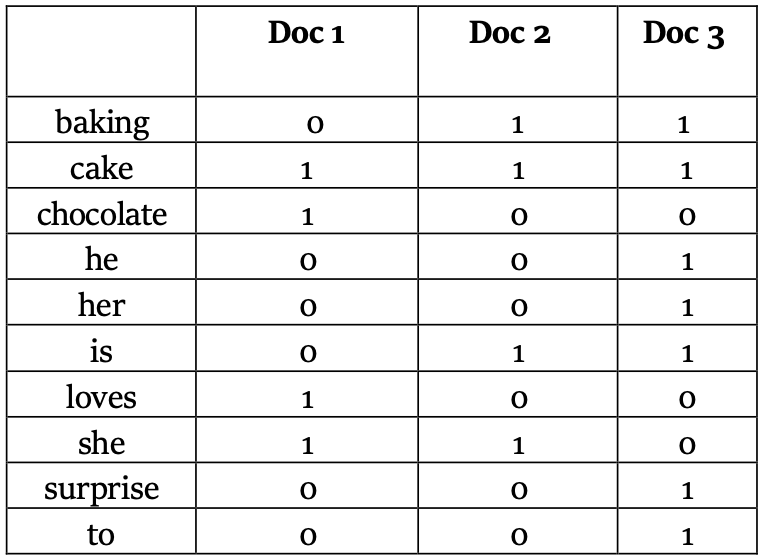
\includegraphics[scale=0.5]{static/table_bow.png}
        \caption{\label{fig:table_bow} Bag-of-words Sparse Matrix \cite{Buddhadev2025}}
    \end{subfigure}
    \begin{subfigure}{0.5\textwidth}
        \centering
        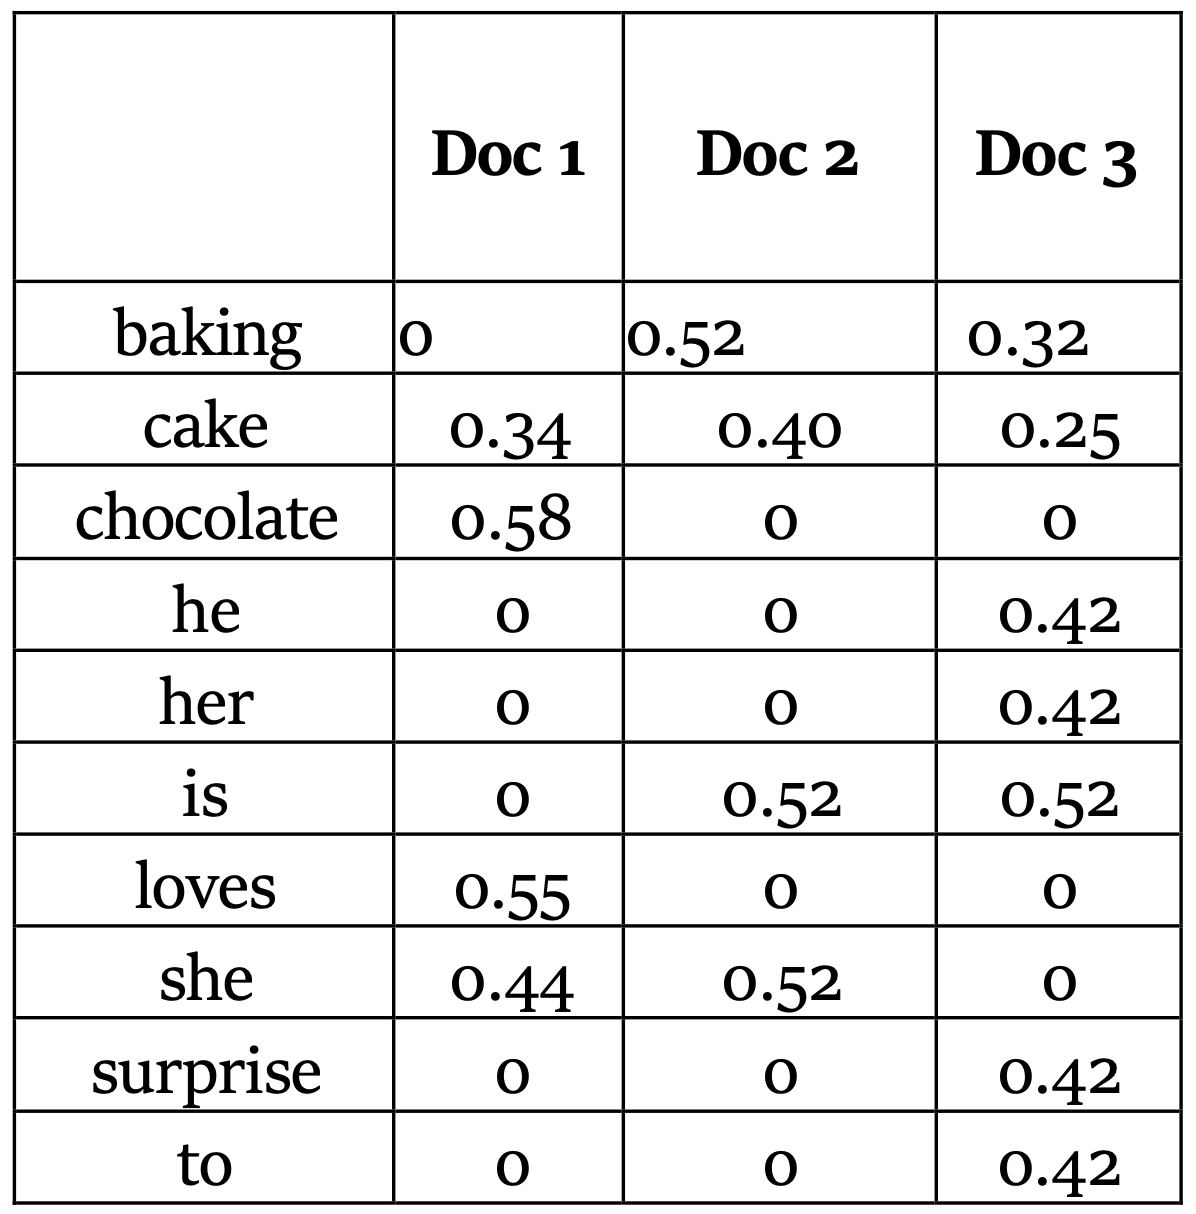
\includegraphics[scale=0.25]{static/table_tf-idf.png}
        \caption{\label{fig:table_tf-idf} TF-IDF Sparse Matrix \cite{Buddhadev2025}}
    \end{subfigure}
    
    \caption{Vergleich der Sparse Matrizen}
    \label{fig:vlg_sparse_matrizen}
\end{figure}

In Abbildung \ref{fig:vlg_sparse_matrizen} wurden den beiden Matrizen jeweils die drei Dokumente:

\begin{itemize}
    \item Doc1 - She loves chocolate cake
    \item Doc2 - She is baking a cake
    \item Doc3 - He is baking a cake to surprise her
\end{itemize}

hinzugefügt. In der Matrix \ref{fig:table_bow} werden in jeder Zelle in welcher das Dokument das entsprechende Wort beinhaltet eine 1 gesetzt.
In \ref{fig:table_tf-idf} wird statt einer 1 eine Gewichtung über die Häufigkeit der Wörter in allen Dokumenten hinweg erstellt und eingetragen.
Sie bewertet die Wichtigkeit eines Wortes in einem Dokument relativ zur gesamten Sammlung von Dokumenten. Dabei wird die Termfrequenz (TF) mit der 
invertierten Dokumentfrequenz (IDF) multipliziert. Je höher der resultierende Wert, desto relevanter ist das Wort für das jeweilige Dokument. 
Die Formel lautet:

\begin{equation}
    \text{tfidf}(t, d, D) = \text{tf}(t, d) \cdot \text{idf}(t, D)
\end{equation}

Dabei ist \( t \) das Wort, \( d \) das Dokument und \( D \) die gesamte Dokumentensammlung \cite{aslam2022}.

Die TF misst, wie häufig ein bestimmter Begriff \( t \) in einem Dokument \( d \) vorkommt. 
Sie beschreibt die lokale Bedeutung eines Wortes innerhalb des Dokuments.

\begin{equation}
\text{tf}(t, d) = \frac{\text{Anzahl der Vorkommen von } t \text{ in } d}{\text{Gesamtanzahl der Wörter in } d}
\end{equation}

Die IDF bewertet, wie selten ein Begriff \( t \) in der gesamten Dokumentensammlung \( D \) ist. 
Je seltener ein Begriff in vielen Dokumenten vorkommt, desto höher ist sein IDF-Wert.

\begin{equation}
    \text{idf}(t, D) = \log \left( \frac{N}{\text{df}(t)} \right)
\end{equation}

Dabei ist \( N \) die Gesamtanzahl der Dokumente in der Matrix und \( \text{df}(t) \) die Anzahl der Dokumente, 
in denen der Begriff \( t \) vorkommt \cite{qaiser2018}.

Die in \cite{Domenico2016} beschriebene Relevance Frequency (RF) ist eine überwachte Gewichtungsform der IDF-Komponente im TF-IDF, die nicht nur zählt, 
in wie vielen Dokumenten ein Begriff vorkommt, sondern berücksichtigt, in welchen Klassen der Begriff besonders häufig oder exklusiv ist.
Die Formel lautet:

\begin{equation}
    \text{rf}(t) = \log\left(2 + \frac{P(t)}{\max(1, N(t))} \right)
\end{equation}

Mit \( P(t) \) für die Anzahl der relevanten Dokumente (z.\,B. positive Klasse), in denen der Term \( t \)
und \( N(t) \) für die Anzahl der irrelevanten Dokumente (z.\,B. negative Klasse), in denen der Term \( t \) vorkommt.

Während klassisches IDF ein Wort umso höher gewichtet, je seltener es allgemein in der Gesamtmatrix ist,
gewichtet RF hingegen ein Wort umso höher, je stärker es mit einer bestimmten Zielklasse assoziiert ist.
Dadurch hebt RF Begriffe hervor, die klassenunterscheidend sind was beim Arbeiten mit überwachten Modellen relevant ist.

In der IF-IDF wird für IDF wird nun also RF eingesetzt und es ergibt sich folgende Formel:

\begin{equation}
    \text{tfidf}(t, d) = \frac{\text{Anzahl der Vorkommen von } t \text{ in } d}{\text{Gesamtanzahl der Wörter in } d} \cdot \log\left(2 + \frac{P(t)}{\max(1, N(t))} \right)
\end{equation}

\begin{itemize}
    \item Mit dem Wort \( t \) und dem Dokument \( d \) 
    \item \( P(t) \) für die Anzahl der relevanten Dokumente (z.\,B. positive Klasse), in denen der Term \( t \) vorkommt
    \item \( N(t) \) für die Anzahl der irrelevanten Dokumente (z.\,B. negative Klasse), in denen der Term \( t \) vorkommt
\end{itemize}

\subsubsection{Vergleich Bag-of-words und TF-IDF}

\begin{table}[!ht]
    \renewcommand{\arraystretch}{1.3}
    \centering
        \begin{tabular}{|p{6.6cm}|p{6.6cm}|}
            \hline
            \textbf{Bag-of-Words (BoW)} & \textbf{TF-IDF} \\
            \hline
            Einfache Implementierung \cite{cichosz2018forum} & Berücksichtigt Wortwichtigkeit in gesamter Matrix  \cite{elov2023uzbek} \\
            \hline
            Keine Gewichtung — häufige Wörter dominieren & Seltener, aber informativer Inhalt wird stärker gewichtet \cite{das2023tfidf} \\
            \hline
            Hohe Dimensionalität in Sparse Matrix (jedes Wort bekommt eine separate Dimension) \cite{ibm_bow} & Gleiches Problem, aber mit informativeren Werten \cite{alzami2020tfidf} \\
            \hline
            Ignoriert Wortreihenfolge und Kontext \cite{umar2022sentiment} & Gleiches Grundproblem, aber geringfügig bessere Performance \cite{parmar2024stacking} \\
            \hline
            Nützlich für einfache Klassifikatoren & Bessere Klassifikationsergebnisse in Kombination mit SVM oder Logistic Regression \cite{iyer2024sentiment} \\
            \hline
        \end{tabular}
    \caption{Vergleich der Vor- und Nachteile von BoW und TF-IDF} %TODO: ChatGPT ?
    \label{tab:vergleich}
\end{table}

Aus Tabelle \ref{tab:vergleich} zu erkennen ist, dass TF-IDF in vielen Anwendungen leistungsfähiger ist als BoW. Insbesondere bei Texten mit hohem Vokabularumfang.

\subsubsection{Hashing Vectorizer}

Ein Hashing Vectorizer ist eine Methode zur Umwandlung von Text in numerische Merkmalsvektoren, ohne dass ein Vokabular explizit 
erstellt oder gespeichert wird. Stattdessen wird eine Hash-Funktion verwendet, um jedes Wort auf einen Index im Feature-Vektor abzubilden \cite{Buddhadev2025}.

In Abbildung \ref{fig:vgl_bow_tfidf_hashing} wird der Vergleich zwischen Machine-Learning-Modellen unter Verwendung von BoW-, TF-IDF- und
Hashing-Features gezeigt. Die y-Achse präsentiert den F1-Score, also die Precision und Recall-Werte der jeweiligen Modelle.
Das Random-Forest-Modell (RF) zeigt eine schwache Leistung bei der Verwendung von Hashing, während die linearen Modelle 
(z.B. SVM (Support Vector Machine) und LR (Logistische Regression)) ihre F1-Werte mit Hashing-Features verbessern konnten. 

Die Verbesserung ist aber nur minimal. Der F1-Score bei SVM ist ohne Hashing bei 0.89 und nach bei 0.90. 
Bei LR steigt der Wert auch von 0.87 und 0.88.

\begin{figure}[htbp]
    \begin{center}
        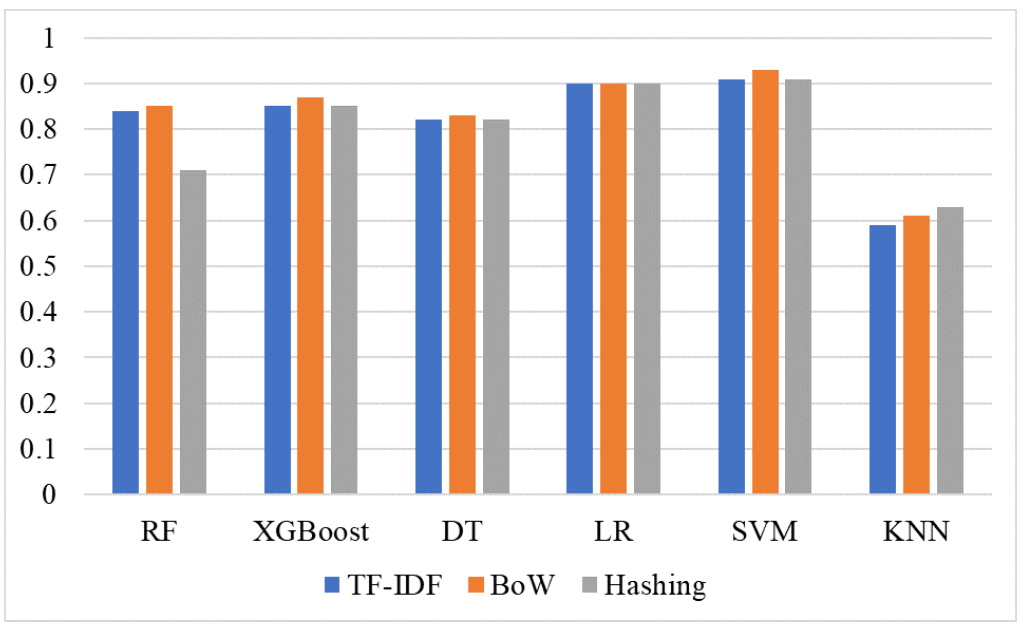
\includegraphics[scale=0.5]{static/bow_vs_tfidf_vs_hashing.png}
        \caption{\label{fig:vgl_bow_tfidf_hashing} Vergleich verschiedener Modelle mit BoW, TF-IDF und Hashing \cite{aslam2022}}
    \end{center}
\end{figure}

\subsection{Machine Learning Modelle}
\label{sec:ml_modelle}

\subsubsection{Naive-Bayes}

Der Naive-Bayes-Algorithmus ist ein einfacher, aber leistungsfähiger Klassifikator, der auf dem Satz von Bayes basiert. 
Er wird häufig in Bereichen wie Textklassifikation, Spam-Erkennung und Sentiment-Analyse eingesetzt \cite{zhang2004}.

Der Klassifikator nutzt den Satz von Bayes zur Berechnung der Wahrscheinlichkeit einer Klasse \( C \) gegeben eine Merkmalsmenge \( X \):

\begin{equation}
    P(C \mid X) = \frac{P(X \mid C) \cdot P(C)}{P(X)}
\end{equation}

Dabei ist:

\begin{itemize}
  \item \textbf{\( P(C \mid X) \)} – \emph{Posterior}: Die Wahrscheinlichkeit für die Klasse \( C \), nachdem die Daten \( X \) beobachtet wurden.
  \item \textbf{\( P(X \mid C) \)} – \emph{Likelihood}: Die Wahrscheinlichkeit, die Daten \( X \) zu sehen, wenn sie zur Klasse \( C \) gehören.
  \item \textbf{\( P(C) \)} – \emph{Prior}: Die ursprüngliche Wahrscheinlichkeit der Klasse \( C \), ohne Kenntnis über die Daten.
  \item \textbf{\( P(X) \)} – \emph{Evidenz}: Die Gesamtwahrscheinlichkeit, die Daten \( X \) zu beobachten (über alle Klassen hinweg).
\end{itemize}

Die zentrale Annahme des Naive-Bayes-Klassifikators ist die bedingte Unabhängigkeit der Merkmale:

\begin{equation}
    P(X \mid C) = \prod_{i=1}^{n} P(x_i \mid C)
\end{equation}

Dies vereinfacht die Berechnung erheblich, da nur die Wahrscheinlichkeiten einzelner Merkmale betrachtet werden müssen \cite{webb2010naive}.

\subsubsection{Decision Tree}

Ein Decision Tree (Entscheidungsbaum) ist ein Algorithmus für Klassifikation und Vorhersage. 
Er basiert auf einer baumartigen Struktur, bei der jeder Knoten bzw. Ast ein Merkmal aus einem Datensatz repräsentiert. 
Diese Struktur ermöglicht es, schrittweise Entscheidungen zu treffen, die schließlich zu einer Klassenzuordnung an einem Blattknoten führen \cite{10.3389/frai.2023.1124553}.

Der Baum wird durch Auswahl von Merkmalen aufgebaut, die die Daten am besten aufspalten. 
Dieses Auswahlkriterium basiert auf dem Konzept der \textbf{Entropie} und dem daraus abgeleiteten \textbf{Informationsgewinn}. 
Ziel ist es, bei jeder Entscheidung im Baum das Merkmal auszuwählen, das die größte Reduktion an Unsicherheit bietet.

Die Entropie misst die Unreinheit oder Unbestimmtheit eines Datensatzes. Sie ist dann maximal, 
wenn alle Klassen gleichverteilt sind, und minimal (d.h. null), wenn alle Daten zur selben Klasse gehören. 
Die Entropie \( E(S) \) eines Datensatzes \( S \) wird wie folgt berechnet:

\begin{equation}
    E(S) = - \sum_{i=1}^{c} p_i \log_2 p_i
\end{equation}

Dabei ist:
\begin{itemize}
  \item \( c \) die Anzahl der Klassen,
  \item \( p_i \) der Anteil der Klasse \( i \) im Datensatz \( S \).
\end{itemize}

Der Informationsgewinn misst die Reduktion der Entropie, die durch das Aufteilen eines Datensatzes mittels eines bestimmten Merkmals erzielt wird. Je größer der Informationsgewinn, desto besser ist das Merkmal für die Aufspaltung geeignet. Eine alternative Formel für den Informationsgewinn $IG(E)$ lautet:

\begin{equation}
    IG(E) = 1 - \sum_{i=1}^{c} p_i^2
\end{equation}

Über einen Hyperparameter kann die maximale Tiefe des Baumes festlegt werden. 
Eine zu große Tiefe kann zu Overfitting führen, da der Baum zu sehr an die Trainingsdaten angepasst wird \cite{aslam2022}.


\subsubsection{Random Forest}

Ein Random Forest besteht aus einer großen Anzahl von Entscheidungsbäumen. 
Jeder Baum wird auf einem zufällig gezogenen Teildatensatz trainiert (Bagging). 
Bei der Bildung jedes Knotens (Split) wird eine zufällige Teilmenge von Merkmalen berücksichtigt. 
Die finale Klassifikation ergibt sich durch Mehrheitsentscheidung aller Bäume (Ensemble Voting) \cite{elchami2025}.

Die Bedeutung eines Merkmals \( i \) im Random Forest ergibt sich aus der durchschnittlichen normierten Bedeutung 
dieses Merkmals über alle Entscheidungsbäume hinweg. Diese kann mathematisch wie folgt dargestellt werden:

\begin{equation}
    RFf_i = \frac{\sum_{j \in \text{all trees}} normf_{ij}}{T}
\end{equation}

Dabei ist:
\begin{itemize}
    \item \( RFf_i \) die Gesamtrelevanz der Klasse \( i \) im gesamten Wald,
    \item \( normf_{ij} \) die normierte Wichtigkeit des Merkmals \( i \) im Baum \( j \),
    \item \( T \) die Gesamtanzahl der Entscheidungsbäume \cite{aslam2022}.
\end{itemize}

Wichtige Hyperparameter sind hier:
\begin{itemize}
    \item \texttt{n\_estimators}: Anzahl der Entscheidungsbäume im Wald.
    \item \texttt{max\_depth}: Maximale Tiefe der Bäume.
    \item \texttt{max\_features}: Anzahl der Merkmale, die für einen Split berücksichtigt werden.
    \item \texttt{bootstrap}: Gibt an, ob Stichproben mit Zurücklegen gezogen werden.
\end{itemize}

Im Vergleich zu Decision Trees ist Random Forest robuster gegenüber Overfitting und bringt durch das Ensemble Voting eine 
höhere Genauigkeit \cite{al-tarawneh2025}.

\subsubsection{Support Vector Machines}

Support Vector Machines (SVMs) sind überwachte Lernalgorithmen, die besonders effektiv für Klassifikationsaufgaben sind. 
Sie finden breite Anwendung in Bereichen wie Bioinformatik, Textklassifikation und 
insbesondere in der Erkennung von Fake News. 
Das Ziel einer SVM ist es, eine Trennlinie --- oder in höherdimensionalen Räumen ein Trenn-Hyperplane --- zu finden, 
das Datenpunkte verschiedener Klassen mit maximalem Abstand (Margin) voneinander trennt  \cite{Noble:2006aa, Buddhadev2025, sabir2025, jakkula2006tutorial}.

\textbf{1. Ziel: Eine Trennebene finden}
Eine SVM sucht eine Gerade (in 2D), Ebene (in 3D) oder Hyperplane, die die Klassen voneinander trennt:
\begin{equation}
w^T x + b = 0
\end{equation}

\textbf{2. Bedingung für korrekte Trennung}
Für jeden Punkt \( x_i \) mit zugehörigem Label \( y_i \in \{-1, +1\} \) gilt:
\begin{equation}
y_i(w^T x_i + b) \geq 1
\end{equation}

\begin{figure}[htbp]
    \begin{center}
        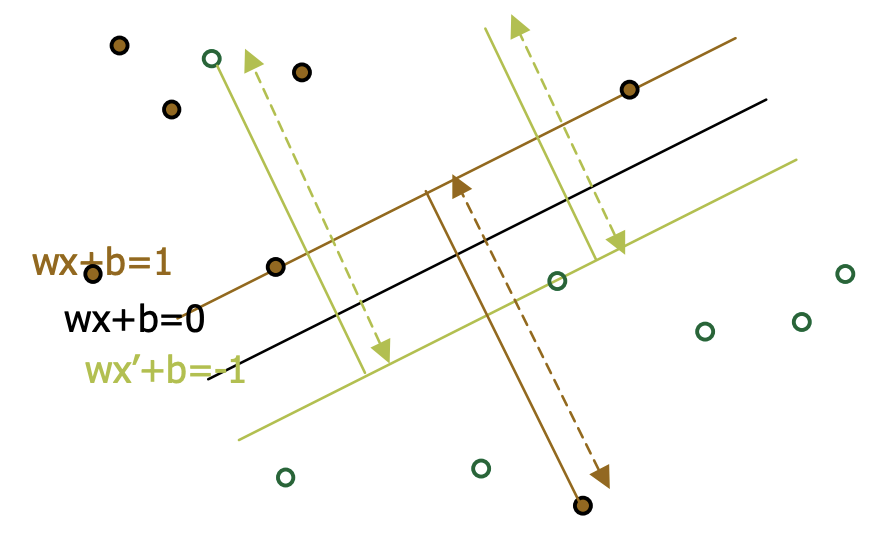
\includegraphics[scale=0.5]{static/fig_hyperplanes.png}
        \caption{\label{fig:hyperplanes} Darstellung von Hyperplanes \cite{jakkula2006tutorial}}
    \end{center}
\end{figure}

\textbf{3. Margin maximieren}
Der Margin ist der Abstand der nächsten Punkte beider Klassen zur Trennebene:
\begin{equation}
M = \frac{2}{\|w\|}
\end{equation}

Daher wird zur Maximierung des Margins folgende Zielfunktion minimiert:
\begin{equation}
\min_{w, b} \quad \frac{1}{2} \|w\|^2
\quad \text{mit} \quad y_i(w^T x_i + b) \geq 1
\end{equation}

\textbf{4. Fehler zulassen – Soft Margin}

Bei nicht perfekt trennbaren Daten werden sogenannte Slack-Variablen \( \xi_i \) eingeführt:
\begin{equation}
y_i(w^T x_i + b) \geq 1 - \xi_i, \quad \xi_i \geq 0
\end{equation}

Ziel ist es, Fehler klein zu halten, gleichzeitig aber den Margin möglichst groß:
\begin{equation}
\min \left( \frac{1}{2} \|w\|^2 + C \sum \xi_i \right)
\end{equation}

\textbf{5. Nichtlineare Trennung – Kernel-Trick}

Bei komplexen Datensätzen wird das Problem durch eine Funktion \( \phi \) in höhere Dimensionen überführt, ohne sie explizit zu berechnen \cite{jakkula2006tutorial}:
\begin{equation}
K(x_i, x_j) = \phi(x_i)^T \phi(x_j) 
\end{equation}

Gängige Kernel-Funktionen:
\begin{itemize}
  \item Linearkernel: \( K(x, x') = x^T x' \)
  \item Polynomial: \( K(x, x') = (x^T x' + 1)^d \)
  \item Radial Basis Function (RBF): \( K(x, x') = \exp(-\gamma \|x - x'\|^2) \) \cite{jakkula2006tutorial}
\end{itemize}
\cite{Noble:2006aa} zeigt, dass durch geeignete Wahl eines Kernels auch komplex strukturierte Daten erfolgreich klassifiziert werden können.

\textbf{Es ergibt sich folgender Ablauf:}

\begin{enumerate}
  \item Definiere Trennebene: \( w^T x + b = 0 \)
  \item Erzwinge korrekte Trennung: \( y_i(w^T x_i + b) \geq 1 \)
  \item Maximiere Margin: \( \min \frac{1}{2} \|w\|^2 \)
  \item Erlaube kleine Fehler: \( \min \frac{1}{2} \|w\|^2 + C \sum \xi_i \)
  \item Wende ggf. Kernel an: \( K(x_i, x_j) = \phi(x_i)^T \phi(x_j) \)
\end{enumerate}

\textbf{Vorteile von SVMs sind:}

\begin{itemize}
    \item \textbf{Robustheit gegenüber Overfitting}, insbesondere bei hoher Dimensionalität und geringem Datensatz \cite{Noble:2006aa}.
    \item \textbf{Gute Generalisierungsfähigkeit} durch Maximierung des Margins.
    \item \textbf{Effizient in der Praxis}: Für viele reale Probleme sind SVMs konkurrenzfähig gegenüber tieferen Netzwerken, (z.B. in Fake-News-Klassifikationen) \cite{Buddhadev2025, sabir2025}.
    \item \textbf{Flexibilität durch Kernel-Funktionen}, womit verschiedene Datentypen (z.B. Vektoren, Strings, Graphen) verarbeitet werden können.
\end{itemize}

\subsubsection{Logistische Regression}

Die logistische Regression (LR) ist ein weit verbreitetes Verfahren des überwachten maschinellen Lernens zur Klassifikation binärer und 
multiklassiger Zielvariablen. Sie wird eingesetzt, um die Wahrscheinlichkeit zu berechnen, mit der eine Beobachtung zu einer 
bestimmten Klasse gehört \cite{elchami2025, aslam2022, SUDHAKAR2024101028}. Im Gegensatz zur linearen Regression verwendet LR eine Aktivierungsfunktion, 
typischerweise die Sigmoidfunktion, um Ausgaben zwischen 0 und 1 abzubilden. Diese Werte stellen Wahrscheinlichkeiten dar und werden zur 
Vorhersage diskreter Zielwerte genutzt \cite{aslam2022}. Die Tabelle \ref{tab:linkfunktionen} zeigt die Aktivierungsfunktionen, mit deren entsprechend
benötigten Zielvariablen.

\begin{table}[ht]
        \renewcommand{\arraystretch}{1.3}
    \centering
        \begin{tabular}{|p{4.4cm}|p{4.4cm}|p{4.4cm}|}
        \hline
        \textbf{Typ} & \textbf{Aktivierungsfunktion} & \textbf{Typ der Zielvariable}\\
        \hline
        Binäre logistische Regression & Logit (Sigmoid): $\frac{1}{1 + e^{-z}}$ & Binär (0/1) \\
        \hline
        Multinomiale logistische Regression & Softmax: $\frac{e^{z_k}}{\sum_j e^{z_j}}$ & Kategorisch (mehrere Klassen) \\
        \hline
        Ordinale logistische Regression & Cumulative Logit, Probit, Cloglog & Geordnete Klassen \\
        \hline
        Probit-Modell & $\Phi(z)$ (Normalverteilung) & Binär (0/1), robust gegen Ausreißer \\
        \hline
        \end{tabular}
\caption{Übersicht von Aktivierungsfunktion in der logistischen Regression \cite{jurafsky2023, hastie2009, agresti2018cda}}
\label{tab:linkfunktionen}  %TODO: ChatGPT ?
\end{table}

Das Ziel der logistischen Regression ist es, eine Funktion zu finden, die die Wahrscheinlichkeit \( P \) berechnet, 
dass ein Eingabewert \( X \) zur Klasse \( y = 1 \) gehört. Dies geschieht zum Beispiel mittels der Sigmoidfunktion \cite{jurafsky2023}:

\begin{equation}
    P = \frac{1}{1 + e^{-(a + bX)}}
\end{equation}

Dabei sind:
\begin{itemize}
  \item \( P \): Wahrscheinlichkeit für Klasse 1 (Wert zwischen 0 und 1)
  \item \( X \): Eingabewert (Merkmalsvariable)
  \item \( b \): Gewicht des Merkmals
  \item \( a \): \textbf{Bias} oder \textbf{Intercept}, also der Schnittpunkt mit der y-Achse, verschiebt die Entscheidungsgrenze. 
  Ohne Bias würde die Entscheidungsgrenze immer durch den Ursprung laufen, was in der Praxis selten sinnvoll ist \cite{geron2019}.
\end{itemize}

In \cite{elchami2025} wurde der Intercept explizit deaktiviert, wodurch sich die Gleichung zu \( P = 1 / (1 + e^{-bX}) \) vereinfacht.

\textbf{Vorteile der logistischen Regression:}
\begin{itemize}
  \item \textbf{Einfachheit und Interpretierbarkeit}: LR-Modelle sind leicht verständlich und liefern direkt interpretierbare Wahrscheinlichkeiten \cite{aslam2022}.
  \item \textbf{Effizienz}: Sie sind schnell trainierbar und benötigen relativ geringe Rechenleistung \cite{SUDHAKAR2024101028}.
  \item \textbf{Flexibilität}: LR lässt sich für binäre, multinomiale und ordinale Klassifikationsprobleme erweitern \cite{SUDHAKAR2024101028}.
  \item \textbf{Breite Anwendbarkeit}: Sie wird in zahlreichen Bereichen eingesetzt, von der Medizin bis zur Textklassifikation \cite{aslam2022, elchami2025}.
\end{itemize}

\subsubsection{K-Nearest Neighbor}

Der K-Nearest Neighbor (KNN) Algorithmus ist ein überwachter Lernalgorithmus, der unter anderem für Klassifikationsprobleme eingesetzt wird. 
Er gehört zur Gruppe der sogenannten lazy learners, da kein expliziter Trainingsprozess stattfindet. 
Stattdessen wird der Trainingsdatensatz während der Vorhersage verwendet \cite{Verma:2024aa}.

KNN klassifiziert neue Instanzen auf Basis ihrer Ähnlichkeit mit bereits bekannten Beispielen. 
Dazu berechnet es die Distanz zwischen dem Testpunkt und allen Trainingspunkten. 
Anschließend werden die \( K \) ähnlichsten Punkte ausgewählt und die Vorhersage erfolgt bei Klassifikation durch 
Mehrheitsentscheidung \cite{aslam2022}.

Die Distanzmessung erfolgt in der Regel über die \textbf{euklidische Distanz}, mit der gemessen wird, 
wie weit zwei Punkte im Merkmalsraum voneinander entfernt sind. Die Formel lautet:

\begin{equation}
    E_d = \sqrt{ \sum_{i=1}^{k} (x_i - y_i)^2 }
\end{equation}

Dabei sind:
\begin{itemize}
    \item \( x_i \): der \( i \)-te Wert des zu klassifizierenden Punkts
    \item \( y_i \): der entsprechende \( i \)-te Wert eines bekannten Trainingspunkts
    \item \( k \): die Anzahl der Merkmale (Dimensionen), z.B. bei Textdaten die Länge des Vektors
\end{itemize}

Je kleiner der Wert \( E_d \), desto ähnlicher sind sich die beiden Punkte.

Der KNN-Algorithmus verwendet mehrere wichtige Hyperparameter:

\begin{enumerate}
    \item \textbf{n\_neighbors}: Gibt an, wie viele der nächsten Trainingspunkte zur Klassifikation berücksichtigt werden. 
    Der Wert (oft als \( K \) bezeichnet) sollte basierend auf den Eigenschaften des Datensatzes gewählt werden \cite{Verma:2024aa, aslam2022}.

    \item \textbf{weights}: Bestimmt, ob allen Nachbarn das gleiche Gewicht gegeben wird oder ob näher gelegene Punkte stärker 
    gewichtet werden \cite{knnparams2024}.

    \item \textbf{metric}: Die Distanzmetrik zur Berechnung der Ähnlichkeit. Standardmäßig wird die euklidische Distanz verwendet, 
    möglich sind aber auch Manhattan, Minkowski oder andere Metriken \cite{aslam2022}
\end{enumerate}

Auch wenn KNN einfach und intuitiv zu implementieren ist und keinen Trainingsprozess benötigt, zeigt Abbildung \ref{fig:nlp_models}, 
dass es im Vergleich mit Naive Bayes (NB), logistischer Regression (LG) und Support Vector Machines (SVM) ein vergleichsweise ineffektives Model 
für NLP ist.

\begin{figure}[htbp]
    \begin{center}
        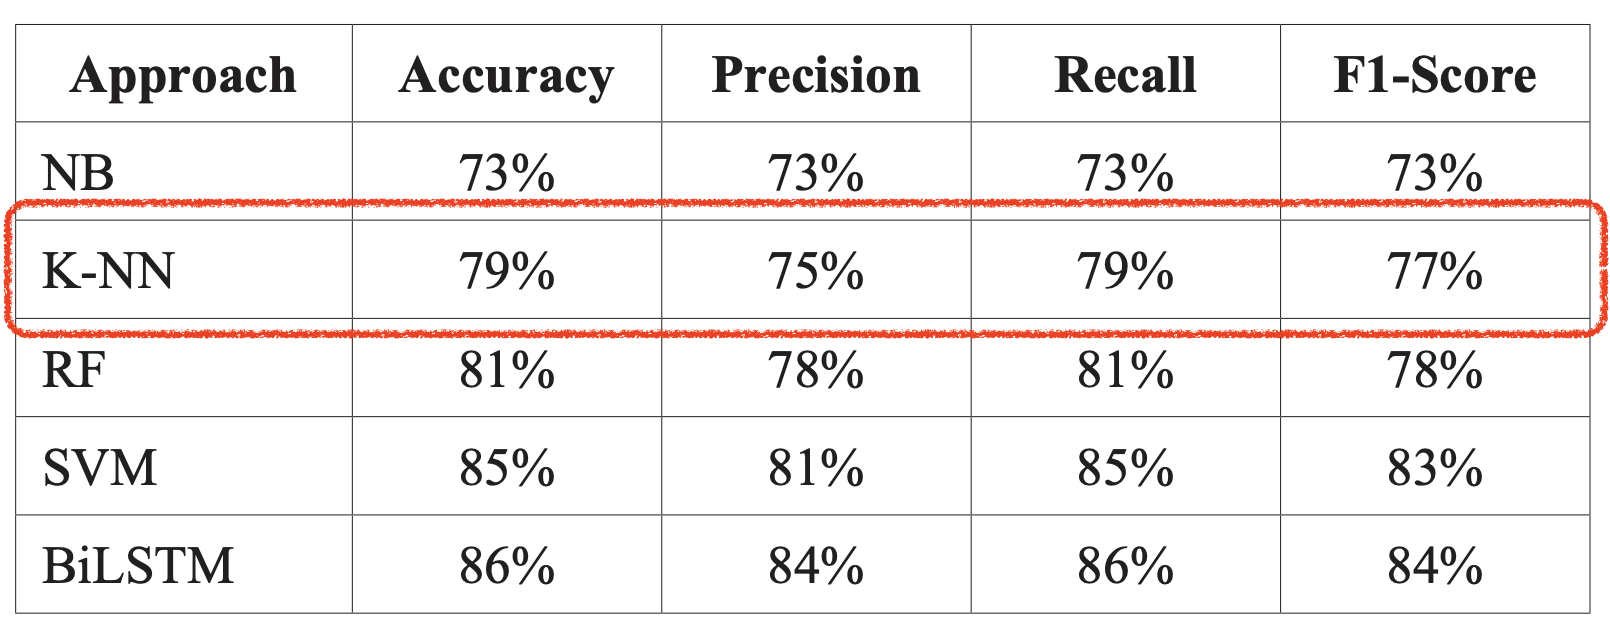
\includegraphics[scale=0.4]{static/vgl_svm_knn_etc.png}
        \caption{\label{fig:nlp_models} Auswertung verschiedener NLP Algorithmen \cite{prom2024}}
    \end{center}
\end{figure}

Hier wurde KNN zur Klassifikation in einem Stimmungserkennungs-System für die Amtssprache Kambodschas eingesetzt. 
Dabei diente KNN dem Vergleich mit anderen Ansätzen wie SVM und wurde insbesondere hinsichtlich seiner Leistung bei der 
Klassifikation von Textdaten bewertet, bei denen die Reihenfolge, der Zeitpunkt oder der Verlauf über die Zeit eine wichtige Rolle 
für die Interpretation und Analyse spielt.

\subsubsection{XGBoost}

eXtreme Gradient Boosting (XGBoost) ist eine Implementierung von Gradient Boosting Decision Trees (GBDT).
Beim XGBoost wird das Modell durch die Addition mehrerer Entscheidungsbäume aufgebaut, welche als
schwache Lernalgorithmen (base learners) fungieren. 
Anders als bei Random Forests, bei denen Bäume unabhängig voneinander trainiert und aggregiert werden, 
lernen die Bäume in XGBoost aufeinander aufbauend (siehe Abbildung \ref{fig:xgboost}). Die Vorhersage für ein Beispiel ergibt sich aus der Summe der 
Ausgaben aller zuvor gelernten Bäume. Dadurch entsteht ein starkes Modell, das schrittweise durch Fehlerkorrektur 
verbessert wird \cite{petrovic2024,chen2016xgboost,aslam2022}.

\begin{figure}[htbp]
    \begin{center}
        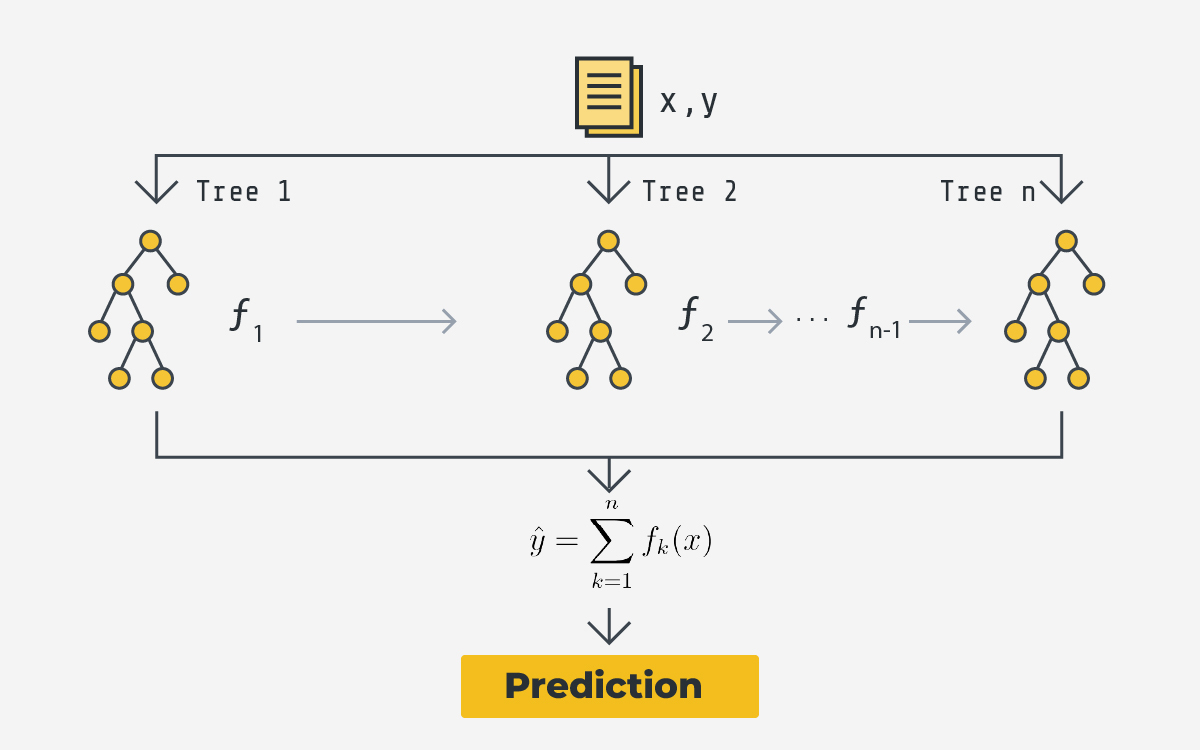
\includegraphics[scale=0.25]{static/xgboost-pipeline.jpg}
        \caption[XGBoost]{\label{fig:xgboost} XGBoost\footnotemark}
    \end{center}
\end{figure}
\footnotetext{\url{https://flower.ai/blog/2023-11-29-federated-xgboost-with-bagging-aggregation/}} %TODO: remove footnote

Ein zentraler Vorteil von XGBoost ist die integrierte Regularisierung, mit der das Modell Overfitting vermeiden kann. 
Dabei werden zwei Arten von Regularisierung eingesetzt:

\begin{itemize}
    \item \textbf{L1-Regularisierung}: Bestraft große Gewichtswerte, indem sie einige Gewichte auf Null setzt. 
        Dadurch hilft sie, unwichtige Merkmale automatisch zu entfernen.
    \item \textbf{L2-Regularisierung}: Bestraft extreme Gewichtswerte, ohne sie komplett zu eliminieren. 
        Dies führt zu stabileren Modellen mit kleinen, gleichmäßigen Gewichten.
\end{itemize}

Beide Regularisierungen sind in die sogenannte Ziel- oder Kostenfunktion eingebettet, die das Modell bei jedem Trainingsschritt minimiert. 

In Anwendungen der natürlichen Sprachverarbeitung (NLP) hilft diese Kombination, besonders bei großen Textmerkmalräumen (z.B. TF-IDF), 
relevante Merkmale herauszufiltern und gleichzeitig stabile Modelle zu trainieren\cite{chen2016xgboost}.

\subsubsection{LightGBM}

Das von \cite{ke2017} entwickelte Modell \textit{Light Gradient-Boosting Machine (LightGBM)} ist eine hocheffiziente Implementierung eines GBDT. 
In Bezug auf dieses Modell wurden zwei zentrale Innovationen eingeführt, um das Training bei großen und hochdimensionalen Datensätzen zu beschleunigen, 
ohne die Modellgenauigkeit zu beeinträchtigen:

\paragraph{Gradient-based One-Side Sampling (GOSS)} reduziert den Rechenaufwand von GBDT, indem es nur einen Teil der Dateninstanzen für die Berechnung 
der Informationsgewinne nutzt. Instanzen mit großen Gradienten (hohem Fehler) werden vollständig beibehalten, während aus den Instanzen mit kleinen 
Gradienten eine Stichprobe gezogen wird. Ein Gewichtungsschritt stellt sicher, dass die Verteilung der Daten korrekt bleibt. Dies führt zu einer
deutlich schnelleren Trainingszeit bei nahezu gleichbleibender Genauigkeit.

\paragraph{Exclusive Feature Bundling (EFB)} adressiert das Problem vieler hochdimensionaler Datensätze, in denen viele Merkmale nur selten 
(sogenannte \textit{sparse} Features) oder nie gleichzeitig (\textit{mutually exclusive}) aktiv sind. 
\textit{Sparse} bedeutet, dass die meisten Werte in einem Merkmal Null sind, während \textit{mutually exclusive} bedeutet, dass bestimmte Merkmale sich 
gegenseitig ausschließen – also nicht gleichzeitig einen von Null verschiedenen Wert annehmen. 
EFB fasst solche Merkmale zu sogenannten Bundles zusammen, wodurch sich die Anzahl der zu verarbeitenden Merkmale stark reduziert. 
Das Bündelungsproblem wird als Graphfärbungsproblem modelliert und mit einem Greedy-Algorithmus angenähert.
Dadurch wird der Histogrammaufbau effizienter und das Training insgesamt beschleunigt.

Im Vergleich zu XGBoost, welches die Bäume gleichmäßig pro Ebene aufbaut, wählt LightGBM bei jedem Schritt das Blatt mit dem höchsten Fehler zur Aufspaltung
(siehe Abbildung \ref{fig:lightgbm_vs_xgboost}). Das kann bei LightGBM zu tiefen, asymmetrischen Baumstrukturen führen.

\begin{figure}[htbp]
    \begin{center}
        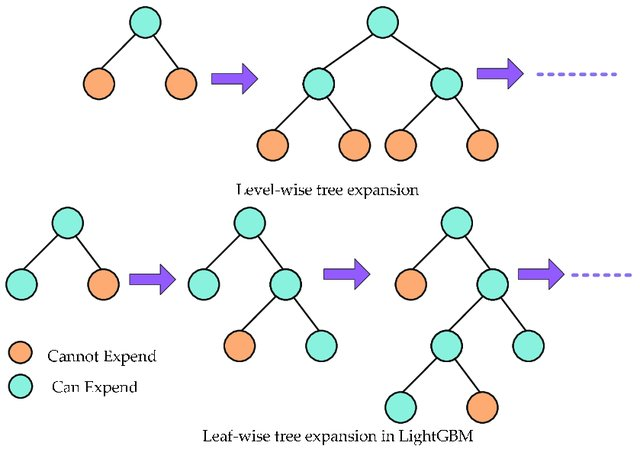
\includegraphics[scale=1.5]{static/lightgbm_vs_xgboost.jpg}
        \caption{\label{fig:lightgbm_vs_xgboost} \textit{level-wise} (XGBoost) vs. \textit{leaf-wise} (LightGBM) \cite{sheng2022}}
    \end{center}
\end{figure}

Folgendes Beispiel einer Fake News Klassifizierung zum Verständnis der Funktionsweise von LightGBM:
\begin{enumerate}
    \item \textbf{Startschätzung:}  
    Das Modell beginnt ohne Entscheidungsbäume. Es trifft eine einfache Anfangsschätzung, z.B. dass jeder Artikel mit gleicher Wahrscheinlichkeit echt 
    oder gefälscht ist (z.B. 50:50-Verteilung).

    \item \textbf{Fehleridentifikation:}  
    Es wird überprüft, welche Artikel falsch klassifiziert wurden. Zum Beispiel: Ein Artikel mit dem Titel „\emph{SCHOCKIEREND: Politiker gesteht alles!}“ 
    wird fälschlicherweise als echt eingestuft, obwohl es sich um eine Falschmeldung handelt.

    \item \textbf{Erzeugung eines ersten Entscheidungsbaums:}  
    Basierend auf den erkannten Fehlern wird der erste Baum trainiert, um die fehlerhaften Vorhersagen zu korrigieren. 
    Dabei lernt das Modell etwa, dass reißerische Sprache mit Fake News korreliert.

    \item \textbf{Anpassung der Vorhersage:}  
    Das Modell passt seine ursprüngliche Schätzung anhand der Regeln des neu erzeugten Baums an. Dieser Baum liefert eine kleine Korrektur, die – 
    positiv oder negativ – zur bestehenden Vorhersage hinzugefügt wird. So wird die Bewertung des Artikels differenzierter und genauer.

    \item \textbf{Weitere Iterationen und Baum-Erzeugung:}  
    Nach jeder Anpassung wird erneut überprüft, wo Fehler verbleiben. Ein weiterer Baum wird erzeugt, um diese Fehler zu korrigieren. 
    Dieser Vorgang wird iterativ wiederholt.

    \item \textbf{Fertiges Modell:}  
    Das finale Modell besteht aus der Summe aller trainierten Bäume. Neue Artikel durchlaufen sämtliche Entscheidungsbäume, 
    deren kombinierte Vorhersagen ergeben eine Wahrscheinlichkeitsaussage.
\end{enumerate} %TODO: ChatGPT

Sowohl \cite{ke2017} als auch \cite{hu2020} zeigen, dass LightGBM gegenüber XGBoost effizienter trainiert, eine bessere Vorhersage gibt, weniger
Merkmale benötigt und kategorische Daten einfacher bearbeiten kann.